%%%%%%%%%%%%%%%%%%%%%%%%%%%%%%%%%%%%%%%%%%%%%%%%%%
%%%%%%%%%%%%%%%%%%%%%%%%%%%%%%%%%%%%%%%%%%%%%%%%%%
%%%%%%%%%%%%%%%%%%%% Required %%%%%%%%%%%%%%%%%%%%
%%%%%%%%%%%%%%%%%%%%%%%%%%%%%%%%%%%%%%%%%%%%%%%%%%
%%%%%%%%%%%%%%%%%%%%%%%%%%%%%%%%%%%%%%%%%%%%%%%%%%

\documentclass[final]{ukthesis} % This calls the ukthesis.cls file, which should be in the same folder.
\usepackage[pdfauthor={Firstname M. Lastname}, % Enter your name here.
            pdftitle={The Dissertation Title}, % Enter your title here.
            pdfsubject={Research Area}, % Enter your research area here.
            pdfkeywords={up, to, six, keywords}, % Enter up to six keywords here.
            pdfproducer={Latex with hyperref},
            pdfcreator={latex->dvips->ps2pdf},
            pdfpagemode=UseOutlines,
            bookmarksopen=true,
            bookmarksnumbered=true]{hyperref}            
\usepackage{memhfixc} % Loading this package here is unnecessary if your hyperref is up to date.


%%%%%%%%%%%%%%%%%%%%%%%%%%%%%%%%%%%%%%%%%%%%%%%%%%
%%%%%%%%%%%%%%%%%%%%%%%%%%%%%%%%%%%%%%%%%%%%%%%%%%
%%%%%%%%%%%%%%%%%%%% Packages %%%%%%%%%%%%%%%%%%%%
%%%%%%%%%%%%%%%%%%%%%%%%%%%%%%%%%%%%%%%%%%%%%%%%%%
%%%%%%%%%%%%%%%%%%%%%%%%%%%%%%%%%%%%%%%%%%%%%%%%%%

\usepackage{amsfonts,amssymb,amsmath,amsthm}
\usepackage[shortlabels]{enumitem}
\usepackage{graphicx,units}
\usepackage{tikz}


%%%%%%%%%%%%%%%%%%%%%%%%%%%%%%%%%%%%%%%%%%%%%%%%%%
%%%%%%%%%%%%%%%%%%%%%%%%%%%%%%%%%%%%%%%%%%%%%%%%%%
%%%%%%%%%%%%%% Bibliography Backend %%%%%%%%%%%%%%
%%%%%%%%%%%%%%%%%%%%%%%%%%%%%%%%%%%%%%%%%%%%%%%%%%
%%%%%%%%%%%%%%%%%%%%%%%%%%%%%%%%%%%%%%%%%%%%%%%%%%

% This template is already set up to use bibtex with the dissertation.bib file.
% If you are most comfortable using bibtex, you can ignore this section.

% I prefer to use biber for the bibliography. It is a robust replacement for bibtex.
% If you would like to use biber, uncomment the below lines and
% swap the Bibliography code at the end of the document.

%\usepackage[backend=biber,style=trad-abbrv]{biblatex}
%\addbibresource{dissertation.bib}

% To configure biber in TexMaker, go to Options -> Configure TexMaker
% and fill the Bib(la)tex field with "biber %".
% You can then go to User -> User Commands -> Edit User Commands and make a custom command.
% I use PdfLatex -> Bibtex -> PdfLatex -> PdfLatex -> View PDF.
% If you use the TeX Live distribution, make sure you have the newest release installed.


%%%%%%%%%%%%%%%%%%%%%%%%%%%%%%%%%%%%%%%%%%%%%%%%%%
%%%%%%%%%%%%%%%%%%%%%%%%%%%%%%%%%%%%%%%%%%%%%%%%%%
%%%%%%%%%%%%%%%% Custom Commands %%%%%%%%%%%%%%%%%
%%%%%%%%%%%%%%%%%%%%%%%%%%%%%%%%%%%%%%%%%%%%%%%%%%
%%%%%%%%%%%%%%%%%%%%%%%%%%%%%%%%%%%%%%%%%%%%%%%%%%

% Put your custom commands here.





















%%%%%%%%%%%%%%%%%%%%%%%%%%%%%%%%%%%%%%%%%%%%%%%%%%
%%%%%%%%%%%%%%%%%%%%%%%%%%%%%%%%%%%%%%%%%%%%%%%%%%
%%%% Front Matter Parameters (fill this out) %%%%%
%%%%%%%%%%%%%%%%%%%%%%%%%%%%%%%%%%%%%%%%%%%%%%%%%%
%%%%%%%%%%%%%%%%%%%%%%%%%%%%%%%%%%%%%%%%%%%%%%%%%%

\begin{document}

\author{Firstname M. Lastname} % Enter your name here as you would like it to be shown.
\title{The Title of the Dissertation} % Enter your title here.

\abstract{ % Put your abstract here.
There should be an abstract here. It is okay if it goes onto the next page, since this occurs in \textbf{Dissertation{\_}Template{\_}12.2018.rtf} (\href{https://uknowledge.uky.edu/uknowledge_docs/11/}{click here}).
}

\advisor{Dr. Doctor McDoctorface} % Enter your advisor's name here, with "Dr." in front.
\keywords{up, to, six, keywords} % Enter up to six keywords for cataloging reasons.
\dgs{Dr. DGS Name} % Enter your DGS's name here, with "Dr." in front.

\frontmatter % This switches the document's page numbering mode.
\maketitle % This currently inserts the cover page, abstract page, and title page. You can change page order in ukthesis.cls.

\begin{dedication} % Optionally enter your dedication here. Otherwise delete.
Dedicated to all math graduate students everywhere.\\
Long have you suffered, but now your time has finally come.\\
This page is optional.
\end{dedication}

\begin{acknowledgments} % Optionally enter your acknowledgements here. Otherwise delete.
\hspace{\parindent}There can optionally be Acknowledgments here. Don't forget to thank your advisor, collaborators, and those who supported you emotionally as well!
\end{acknowledgments}

\pdfbookmark{\contentsname}{toc} % Bookmarks the Table of Contents in the PDF file. This is required.
\tableofcontents*\clearpage % Creates TOC without listing the TOC in the TOC. Required.
\listoftables\clearpage % Required if you have tables.
\listoffigures\clearpage % Required if you have figures.

\mainmatter % This switches the document's page numbering mode.

%%%%%%%%%%%%%%%%%%%%%%%%%%%%%%%%%%%%%%%%%%%%%%%%%%
%%%%%%%%%%%%%%%%%%%%%%%%%%%%%%%%%%%%%%%%%%%%%%%%%%
%%%%%%%%%%%%%%%%%%%%%%%%%%%%%%%%%%%%%%%%%%%%%%%%%%
%%%%%%%%%%%%%%%%%%%%%%%%%%%%%%%%%%%%%%%%%%%%%%%%%%
%%%%%%%%%%%%%%%%%%%%%%%%%%%%%%%%%%%%%%%%%%%%%%%%%%
%%%%%%%%%%%%%%%%%%%%%%%%%%%%%%%%%%%%%%%%%%%%%%%%%%
%%%%%%%%%%%%%%%%%%%% Document %%%%%%%%%%%%%%%%%%%%
%%%%%%%%%%%%%%%%%%%%%%%%%%%%%%%%%%%%%%%%%%%%%%%%%%
%%%%%%%%%%%%%%%%%%%%%%%%%%%%%%%%%%%%%%%%%%%%%%%%%%
%%%%%%%%%%%%%%%%%%%%%%%%%%%%%%%%%%%%%%%%%%%%%%%%%%
%%%%%%%%%%%%%%%%%%%%%%%%%%%%%%%%%%%%%%%%%%%%%%%%%%
%%%%%%%%%%%%%%%%%%%%%%%%%%%%%%%%%%%%%%%%%%%%%%%%%%
%%%%%%%%%%%%%%%%%%%%%%%%%%%%%%%%%%%%%%%%%%%%%%%%%%

\chapter{How to Finish Grad School}

This guide is written by math graduate students, for math graduate students. Please keep it up to date and add any relevant details you learned from your experience. Thanks!

\section{Helpful Pages \& Documents}

Be sure to follow the formatting advice in the following resources and be aware of every deadline. The items below are hyperlinks. Click them to find each document on the web.
\begin{itemize}

\item \href{http://gradschool.uky.edu/key-dates}{Key Dates}

\item \href{https://ris.uky.edu/cfdocs/gs/DoctoralCommittee/Selection_Screen.cfm}{Doctoral Degree Candidate Forms}

\item \href{http://gradschool.uky.edu/electronic-dissertation-defense}{Electronic Dissertation Defense}

\item \href{http://gradschool.uky.edu/electronic-dissertation-preparation}{Electronic Dissertation Preparation}

\item \href{http://gradschool.uky.edu/sites/gradschool.uky.edu/files/Documents/ThesisDissertationPrep/Checklist_Common_Errors_2019.pdf}{The Checklist of Common Errors}

\item \href{http://gradschool.uky.edu/faq-theses-dissertations}{FAQ Theses \& Dissertations}

\item \href{https://uknowledge.uky.edu/cgi/viewcontent.cgi?referer=http://gradschool.uky.edu/electronic-dissertation-defense&httpsredir=1&article=1006&context=uknowledge_docs}{Thesis and Dissertation Submission Guide}

\item \href{https://uknowledge.uky.edu/}{UKnowledge}

\end{itemize}

\section{Steps and Deadlines}

Figure out ahead of time what the following deadlines are. I found it helpful to make a checklist and mark them on my calendar.

\begin{itemize}

\item \textbf{Submit Notification of Intent to Schedule of a Final Doctoral Examination.} This must be submitted a minimum of 8 weeks prior to the anticipated final examination (defense) date.

Note that the defense must take place no later than 8 days prior to the last day of classes of the semester in which you intend to graduate. Plan accordingly.

This step can be done with the Doctoral Degree Candidate Forms (\href{https://ris.uky.edu/cfdocs/gs/DoctoralCommittee/Selection_Screen.cfm}{click here}).

\item \textbf{Submit Request for Final Doctoral Examination.} This must be submitted a minimum of 2 weeks prior to the date of the defense.

This step can be done with the Doctoral Degree Candidate Forms (\href{https://ris.uky.edu/cfdocs/gs/DoctoralCommittee/Selection_Screen.cfm}{click here}).

\item \textbf{Give a copy of the dissertation to your committee.} Do this at the same time you submit the Request for Final Doctoral Examination. (If you're a bit late on this, no one will likely care, but try to do it anyway in the name of professionalism.)

\item \textbf{Defend your dissertation.} You set the date for this with your committee in the previous steps. Check out the room ahead of time and make sure all of the technology is working. Don't be late!

\item \textbf{Complete the Application for Degree on myUK.} This deadline is listed on the Graduate School Calendar (\href{http://gradschool.uky.edu/key-dates}{click here}).

\item \textbf{Submit dissertation for format review on UKnowledge.} You have 60 days to submit this after your defense, or less if the deadline to submit thesis/dissertation for format review (\href{http://gradschool.uky.edu/key-dates}{click here}) is sooner. It will take 2-3 business days to get a response, so plan accordingly. You will most likely have to resubmit with revisions.

Details for submitting this are in the Thesis and Dissertation Submission Guide (\href{https://uknowledge.uky.edu/cgi/viewcontent.cgi?referer=http://gradschool.uky.edu/electronic-dissertation-defense&httpsredir=1&article=1006&context=uknowledge_docs}{click here}).

\item \textbf{Submit a completed ETD Approval Form (\href{http://gradschool.uky.edu/sites/gradschool.uky.edu/files/Forms/StudentForms/ETDApprovalForm_0.pdf}{click here}) as an Additional File on UKnowledge.} You can do this at the same time as your first dissertation submission for format review, or at a later date.

\item \textbf{Submit dissertation revisions on UKnowledge.} The last day to submit revised thesis/dissertation is listed on the Graduate School Calendar (\href{http://gradschool.uky.edu/key-dates}{click here}).

\item \textbf{Submit confirmation of completing the Survey of Earned Doctorates.} Do this with your revision after receiving the result of your format review (even if no revisions are required). The Thesis and Dissertation Submission Guide (\href{https://uknowledge.uky.edu/cgi/viewcontent.cgi?referer=http://gradschool.uky.edu/electronic-dissertation-defense&httpsredir=1&article=1006&context=uknowledge_docs}{click here}) asks you to scan the SED confirmation page at 300dpi. I simply submitted the Certificate of Completion PDF file from the end of the survey, and no one complained.

At this time, you should email your Degree Certification Officer (\href{http://gradschool.uky.edu/academic-affairs-officers}{click here}) to let them know that you have done this step.

\end{itemize}

\section{Formatting Your Dissertation}

In formatting your dissertation, this template along with \textbf{ukthesis.cls} (in the same folder) should handle most of the formatting for you. The \textbf{memoir} class is required. If it is not preinstalled with your {\LaTeX} distribution, you will need to install it. This is most easily done by updating your {\LaTeX} distribution (e.g., TeX Live, MiKTeX, or MacTeX), but the class files are located in the \textbf{Resources} folder if you wish to install them manually.

I ran into some oddities in formatting my dissertation, which I will list here. Please update this document if you discover anything else worth mentioning.

\begin{itemize}
\item Fonts are already embedded in your PDF if you use this template. Additionally, the ``Bookmarks Panel and Page'' is already chosen in Adobe. You will need Adobe Reader (free) or Adobe Acrobat (paid) to minimize the bookmarked chapters so that sections do not appear when the document is opened. See the \href{http://gradschool.uky.edu/sites/gradschool.uky.edu/files/Documents/ThesisDissertationPrep/Checklist_Common_Errors_2019.pdf}{Checklist of Common Errors} for a picture of this. Just click on the arrows and re-save your document. This must be the final step before submitting to UKnowledge.
\item Tables and figures \textbf{must} have captions in order to appear in the List of Tables or List of Figures.
\item Table captions must appear above the table. To do this, simply put the \textbf{caption} command at the top of the \textbf{table} environment.
\item Figure captions may go above or below. I did below, but you do you, boo.
\item Be aware of the table and figure placement requirements on the Electronic Dissertation Preparation page (\href{http://gradschool.uky.edu/electronic-dissertation-preparation#Tables}{click here}). The graduate school is very particular about this.
\item Appendices must be labeled A, B, $\ldots$ and have titles.
\item Tables and figures in appendices have different requirements. See Appendix B for details.
\item Do \textbf{not} use the \textbf{part} environment for separating your content. Chapters and sections are okay.
\item Follow the page order on the Electronic Dissertation Preparation page (\href{http://gradschool.uky.edu/electronic-dissertation-preparation#PageOrder}{click here}). This changes from time to time, so if you need to change it please do so in the \textbf{ukthesis.cls} file. The Editor's Note at the top of the code will tell you how to do so.
\end{itemize}




At the end of each chapter should be a copyright notice. And as always, make sure to cite anything you reference, such as \cite{diffie1976new}.

\copyrightnotice % Required at the end of each chapter


\chapter{Some Math I Guess}

\section{Polyhedra}

A \textbf{polyhedron} is a three-dimensional figure whose faces are all polygons. A polyhedron has \textbf{vertices}, \textbf{edges}, and \textbf{faces}, as shown here:

\begin{figure}[h]
$$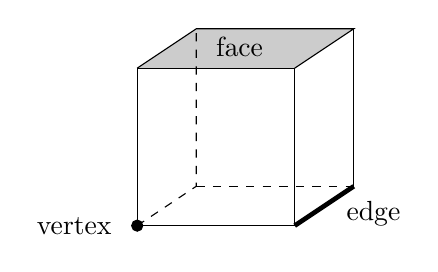
\begin{tikzpicture}
	\draw [dashed] (0, 0) -- (0.75, 0.5) -- (0.75, 2.5);
	\draw [dashed] (0.75, 0.5) -- (2.75, 0.5);
	\path[fill=black, opacity=0.2] (0, 2) -- (2, 2) -- (2.75, 2.5) -- (0.75, 2.5) -- (0, 2);
	\draw (0, 0) -- (2, 0) -- (2, 2) -- (0, 2) -- (0, 0);
	\draw (0, 2) -- (0.75, 2.5) -- (2.75, 2.5) -- (2, 2);
	\draw [line width=0.6mm] (2, 0) -- (2.75, 0.5);
	\draw (2.75, 0.5) -- (2.75, 2.5);
	\filldraw (0, 0) circle (2pt);
	\node at (-0.8, 0) {vertex};
	\node at (3, 0.15) {edge};
	\node at (1.3, 2.275) {face};
\end{tikzpicture}$$
\caption{A cube has 8 vertices, 12 edges, and 6 faces}
\end{figure}

Here are some more polyhedra:

\begin{figure}[h]
$$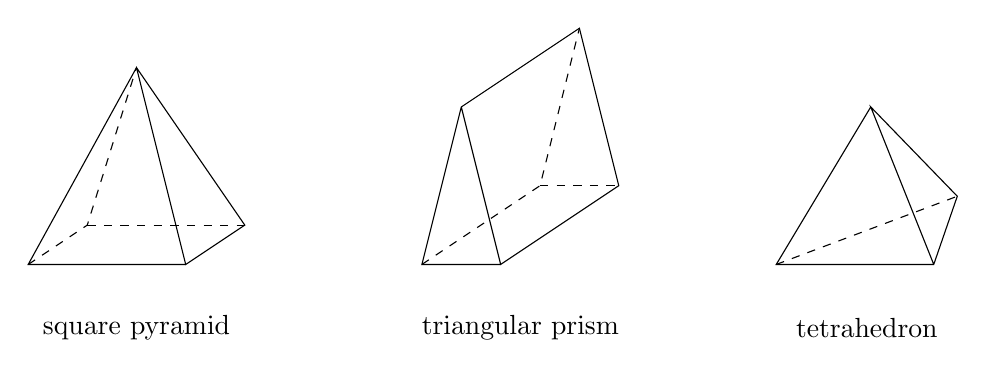
\begin{tikzpicture}
	\draw [dashed] (0, 0) -- (0.75, 0.5) -- (1.375, 2.5);
	\draw [dashed] (0.75, 0.5) -- (2.75, 0.5);
	\draw (2, 0) -- (0, 0) -- (1.375, 2.5) -- (2, 0) -- (2.75, 0.5) -- (1.375, 2.5);

	\draw [dashed] (5, 0) -- (6.5, 1) -- (7, 3);
	\draw [dashed] (6.5, 1) -- (7.5, 1);
	\draw (6, 0) -- (5, 0) -- (5.5, 2) -- (7, 3) -- (7.5, 1) -- (6, 0) -- (5.5, 2);

	\draw [dashed] (9.5, 0) -- (11.799, 0.866);
	\draw (10.7, 2) -- (9.5, 0) -- (11.5, 0) -- (11.799, 0.866) -- (10.7, 2) -- (11.5, 0);

	\node at (1.375, -0.8) {square pyramid};
	\node at (6.25, -0.8) {triangular prism};
	\node at (10.65, -0.8) {tetrahedron};
\end{tikzpicture}$$
\caption{Examples of polyhedra}
\end{figure}

We organize the numbers of vertices ($V$), edges ($E$), and faces ($F$) into the table below.

\renewcommand{\arraystretch}{1.4}
\begin{table}[h]
\centering
\caption{Computing the Euler characteristic}
\begin{tabular}{||l|c|c|c|c||}
\hline
Polyhedron & ~$V$~ & ~$E$~ & ~$F$~ & $V - E + F$ \\ \hline \hline
cube & 8 & 12 & 6 & 6 \\ \hline
square pyramid & 5 & 8 & 5 & 2 \\ \hline
triangular prism & 6 & 9 & 5 & 2 \\ \hline
tetrahedron & 4 & 6 & 4 & 2 \\ \hline
\end{tabular}
\end{table}
\renewcommand{\arraystretch}{1.0}

For each polyhedron in the table above, the Euler characteristic $V-E+F$ is 2.

\section{The Monty Hall Problem}

You are on the game show \textit{Let's Make a Deal} and the host Monty Hall presents you with three doors to choose from. Behind two of the doors are goats, but behind one of the doors is a new car! Once your decision is made, Monty opens one of the other two doors to reveal a goat. He then offers you a choice: keep the door you originally chose, or switch to the other door which was not opened. Do you make the switch?

Naively, it may seem that the chance of the car being behind either of the two remaining doors is an even 50/50 split. Most people wouldn't switch doors, out of fear or other psychological factors. However, a wise person would switch. In fact, the probability of winning the car if you switch is $\nicefrac{2}{3}$, while the probability of winning if you keep your original door is $\nicefrac{1}{3}$.

In your original choice, there is clearly a $\nicefrac{2}{3}$ chance that you will pick the wrong door, and only a $\nicefrac{1}{3}$ chance that you will pick the correct door. The host would not show you the door with the car, so he is forced to show you a door with a goat. Therefore by switching you are guaranteed to get a goat if you started with the car, and likewise you are guaranteed to get the car if you started with a goat.

\begin{figure}[h]
\centering
\begin{tabular}{ccccc}
			&	& Goat	& $\stackrel{\text{switch}}{\longrightarrow}$ & Car	\\
			& $^{\nicefrac{2}{3}}\nearrow$	& &		&	\\
Your Choice	&	& 		&	& \\
			& $_{\nicefrac{1}{3}}\searrow$	& &		&	\\
			&	& Car	& $\stackrel{\text{switch}}{\longrightarrow}$ & Goat
\end{tabular}
\caption{Probability tree for the Monty Hall problem}
\end{figure}

Probability is in your favor if you make the switch!

In an interview \cite{monty}, Monty Hall explained that he never gave contestants the opportunity to switch doors, so this problem is entirely hypothetical. Nevertheless, his name remains attributed to this phenomenon.


\copyrightnotice % Required at the end of each chapter

\backmatter % This ensures that appendices appear correctly in the Table of Contents.

%%%%%%%%%%%%%%%%%%%%%%%%%%%%%%%%%%%%%%%%%%%%%%%%%%
%%%%%%%%%%%%%%%%%%%%%%%%%%%%%%%%%%%%%%%%%%%%%%%%%%
%%%%%%%%%%%%%%%%%%% Appendices %%%%%%%%%%%%%%%%%%%
%%%%%%%%%%%%%%%%%%%%%%%%%%%%%%%%%%%%%%%%%%%%%%%%%%
%%%%%%%%%%%%%%%%%%%%%%%%%%%%%%%%%%%%%%%%%%%%%%%%%%

\chapter{Appendices}
\begin{appendices}

\section{Appendix A: Title your appendices}

If you have appendices, they must have titles and be labeled alphabetically.


\section{Appendix B: A word about figures}

Figures in an appendix should \textbf{not} appear in the List of Figures. To achieve this, you can use the \textbf{center} environment followed by a \textbf{medskip} for appropriate spacing. I believe that the same applies to tables, although I did not confirm this.

The following polyhedron is called a \textbf{truncated cube}.
\begin{center}
$$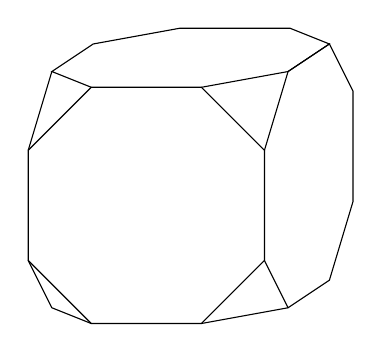
\begin{tikzpicture}
	\draw (0.8, 0) -- (2.2, 0) -- (3, 0.8) -- (3, 2.2) -- (2.2, 3) -- (0.8, 3) -- (0, 2.2) -- (0, 0.8) -- (0.8, 0);
	\draw (3, 2.2) -- (3.3, 3.2) -- (3.825, 3.55) -- (4.125, 2.95) -- (4.125, 1.55) -- (3.825, 0.55) -- (3.3, 0.2) -- (3, 0.8);
	\draw (2.2, 0) -- (3.3, 0.2);
	\draw (2.2, 3) -- (3.3, 3.2);
	\draw (0.8, 0) -- (0.3, 0.2) -- (0, 0.8);
	\draw (0.8, 3) -- (0.3, 3.2) -- (0.825, 3.55) -- (1.925, 3.75) -- (3.325, 3.75) -- (3.825, 3.55) -- (3.3, 3.2);
	\draw (0, 2.2) -- (0.3, 3.2);
\end{tikzpicture}$$
\end{center}
\begin{center}
Figure B1: A truncated cube
\end{center}
\medskip

Furthermore, figures in Appendix A should be labeled A1, A2, $\ldots$ and figures in Appendix B should be labeled B1, B2, $\ldots$.

\end{appendices}


%%%%%%%%%%%%%%%%%%%%%%%%%%%%%%%%%%%%%%%%%%%%%%%%%%
%%%%%%%%%%%%%%%%%%%%%%%%%%%%%%%%%%%%%%%%%%%%%%%%%%
%%%%%%%%%%%%%%%%%% Bibliography %%%%%%%%%%%%%%%%%%
%%%%%%%%%%%%%%%%%%%%%%%%%%%%%%%%%%%%%%%%%%%%%%%%%%
%%%%%%%%%%%%%%%%%%%%%%%%%%%%%%%%%%%%%%%%%%%%%%%%%%

\emergencystretch=2em % This fixes weird justification in the bibliography.

%\printbibliography % This creates the bibliography with biber.

\bibliographystyle{abbrv} % This chooses the bibliography style for bibtex.
\bibliography{dissertation} % This creates the bibliography with bibtex.


%%%%%%%%%%%%%%%%%%%%%%%%%%%%%%%%%%%%%%%%%%%%%%%%%%
%%%%%%%%%%%%%%%%%%%%%%%%%%%%%%%%%%%%%%%%%%%%%%%%%%
%%%%%%%%%%%%%%%% Curriculum Vita %%%%%%%%%%%%%%%%%
%%%%%%%%%%%%%%%%%%%%%%%%%%%%%%%%%%%%%%%%%%%%%%%%%%
%%%%%%%%%%%%%%%%%%%%%%%%%%%%%%%%%%%%%%%%%%%%%%%%%%

\newpage
\chapter{Vita}
\begin{center}
\large{Full Name}
\end{center}

\textbf{Place of Birth:}
\begin{itemize}
\item City, ST
\end{itemize}

\textbf{Education:}
\begin{itemize}
\item University of Kentucky, City, ST\\M.A. in Mathematics, May. 2006
\item Undergraduate University, City, ST\\B.S. in Mathematics, Dec. 2004\\ \textit{cum laude}
\end{itemize}

\textbf{Professional Positions:}
\begin{itemize}
\item Graduate Teaching Assistant, University of Kentucky Fall 2004--Spring 2009
\end{itemize}

\textbf{Honors}
\begin{itemize}
\item Scholarship 1, University of Kentucky
\item Fellowship 1, University of Kentucky
\item Other Recognition or Award, Northern Kentucky University
\end{itemize}

\textbf{Publications \& Preprints:}
\begin{itemize}
\item Puplication 1
\item Preprint 1
\end{itemize}
\end{document}
